\chapter{METODOLOGIAS PARA MEMORIZAÇÃO DE VOCABULÁRIO}
\label{chap:metodologias}
Existem diversos métodos para auxiliar na memorização de novo vocabulário como por exemplo: realizar a leitura da definição de uma palavra repetidas vezes, escrever múltiplas vezes ou até mesmo repetir em voz alta essa palavra e seu significado. O que algumas pesquisas indicam é que repetir o vocabulário enquanto executa algum tipo de exercício físico (escrita ou fala por exemplo) aumenta a capacidade de retenção dos significados das palavras.

\section{Método Dos \textit{Flashcards}}
Um dos métodos mais populares atualmente se baseia em utilizar cartões ou pedaços de papel (\textit{flashcards}) onde de um lado do papel está escrito a palavra que se deseja memorizar na língua estrangeira e do outro lado do papel está a tradução da palavra. A ideia é que o estudante tente lembrar da tradução da palavra sem precisar virar o cartão e para verificar se está correto ele pode facilmente consultar a resposta.

\section{Curva De Esquecimento E Aprendizado }
Em seu livro \textit{Über das Gedächtnis - Memory: A Contribution to Experimental Psychology} o autor Hermann Ebbinghaus (1885 apud TUMELERO, 2018) analisa de forma empírica como as pessoas esquecem a informação depois de adquiri-la. A conclusão obtida foi de que o tempo de esquecimento se comporta de forma exponencial, também chamada de curva de esquecimento (Figura1).

\begin{figure}[H]
\caption{\label{fig:curva_esquecimento}Curva de esquecimento}
\begin{center}
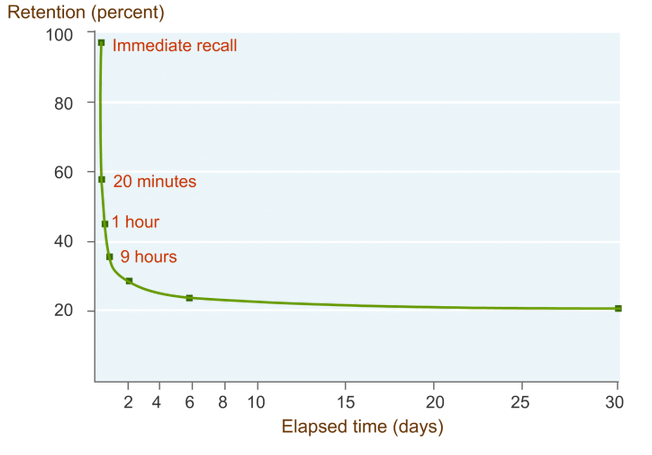
\includegraphics[scale=0.50]{curva_esquecimento}
\end{center}
\legend{Fonte:Disponível em: https://learning-evolution.com. Acesso em: 04 set. 2019.}
\end{figure}

Pode-se notar também que a velocidade com que um estudante esquece as informações depende de múltiplos fatores como dificuldade do tema a ser estudado, como a informação está sendo apresentada e o quão fácil é para o estudante relacionar o conteúdo com algum conhecimento prévio.

O autor ressalta que apesar da velocidade de esquecimento variar, a curva exponencial mantém-se em todas os casos. Baseando-se nessa informação, é também mencionado o efeito causado pelo espaçamento do conteúdo para otimização do aprendizado de algo novo. O estudo revelou que reforçar a informação após um determinado intervalo de tempo é bem mais efetivo do que tentar memorizar uma grande quantidade de informação em um curto período de tempo. 

Em uma pesquisa efetuada em 2007 pela equipe de neurocientistas da \textit{Learning \& Memories}, foi avaliado sob perspectiva biológica e fisiológica a aplicação do princípio de aprendizado espaçado, e percebeu-se que há um maior desenvolvimento dos neurônios na região do hipocampo, que é a região responsável por armazenar memórias a longo prazo.

\begin{figure}[H]
	\caption{\label{fig:memoria_neuro}Aprendizado espaçado aumenta sobrevivência de células no hipocampo}
\begin{center}
	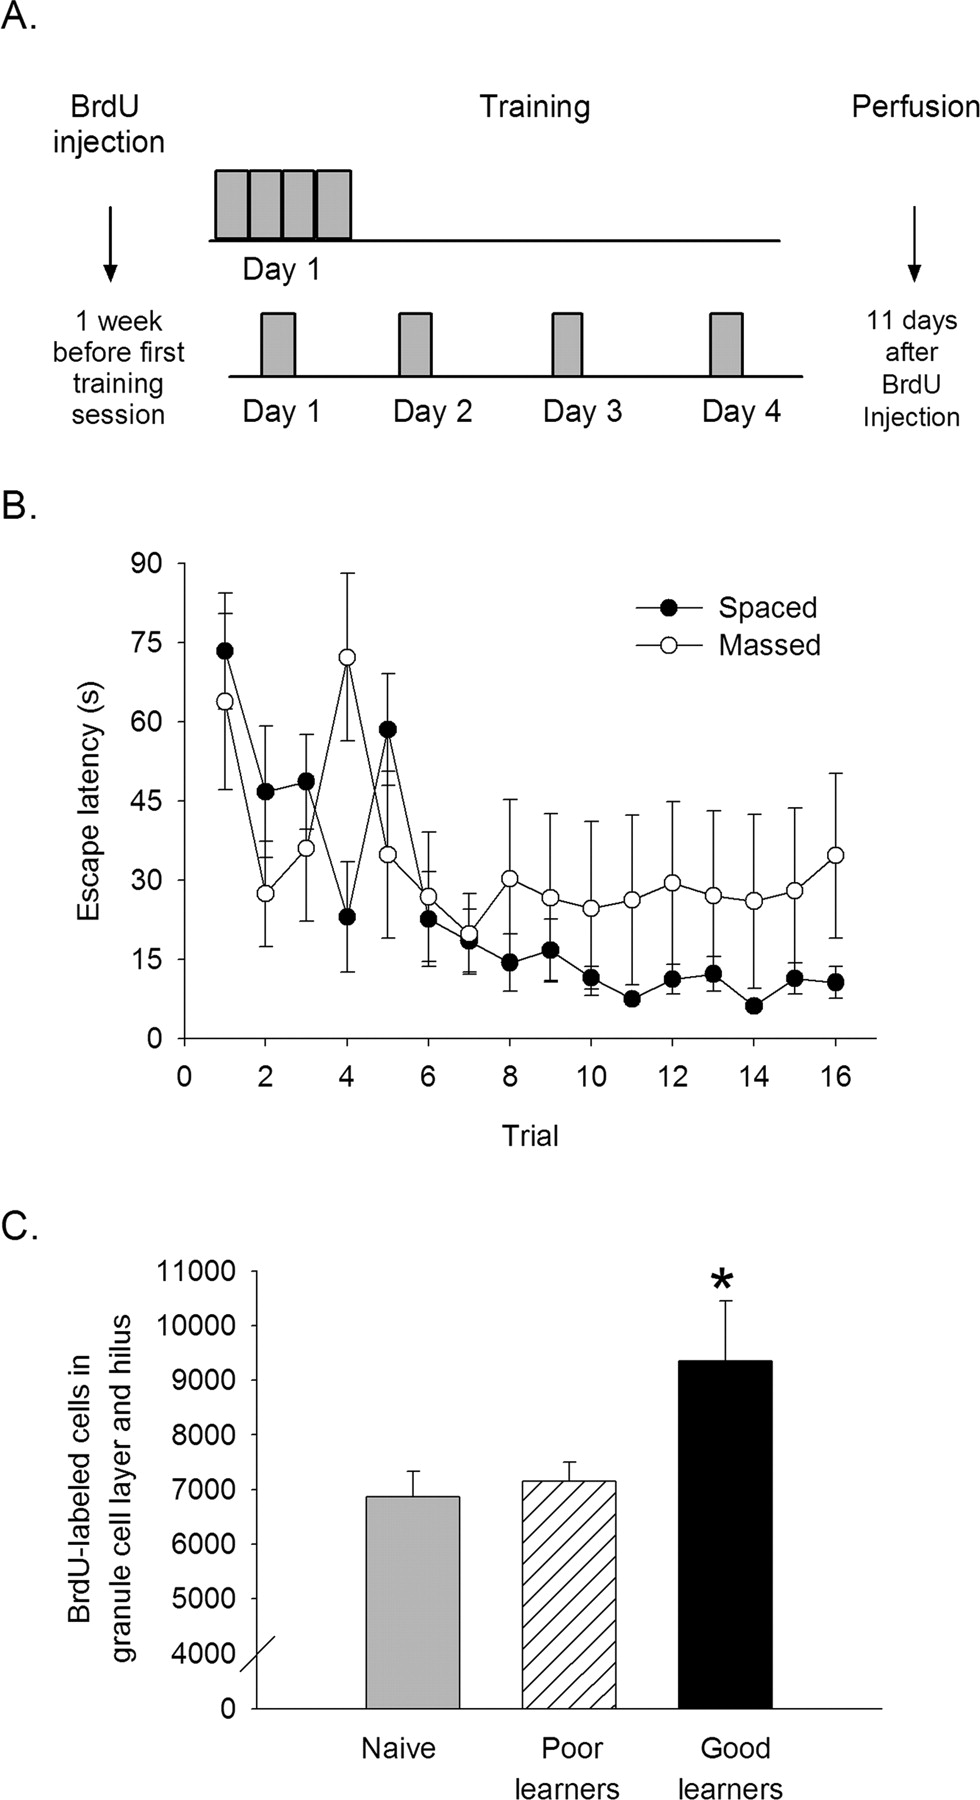
\includegraphics[scale=0.30]{memoria_neuro}
\end{center}
\legend{Fonte: Learning \& Memories - Neurogenesis and the spacing effect: Learning over time enhances memory and the survival of new neurons, 2007.}
\end{figure}

\section{SRS - \textit{Spaced Repetition System}}
Como mencionado anteriormente, o método dos \textit{flashcards} são apenas uma ferramenta para a repetição de conteúdo, o potencial desse método vem de técnicas e algoritmos que utilizam o conceito de aprendizado espaçado. Idealmente o estudante deve estudar de forma otimizada e não repetindo todas as palavras o tempo inteiro, mas apenas repetir as palavras que estiver prestes a esquecer.

Um dos primeiros métodos que utilizou esse princípio para tornar \textit{flashcards} um processo eficiente foi criado por um cientista alemão chamado Sebastian Leitner no ano de 1970 e é conhecido como o Leitner System ou método das caixas (Figura 3). A ideia do método de Leitner era separar esses cartões em diferentes caixas, onde cada caixa é reavaliada de acordo com a familiaridade com os cartões ali contidos. Para cada \textit{flashcard}, se o estudante não lembrar com sucesso da resposta, o cartão é colocado em uma primeira caixa, caso contrário o \textit{flashcard} irá para a caixa seguinte, indicando que o conteúdo foi memorizado. Para cada caixa há um tempo maior no qual o aluno deve revisitar, fazendo assim com que o aluno reavalie com mais frequência os cartões que ele possui mais dificuldade e com menos frequência aqueles que ele já possui domínio.

\begin{figure}[H]
	\caption{\label{fig:leitner_system}Método das caixas}
	\begin{center}
		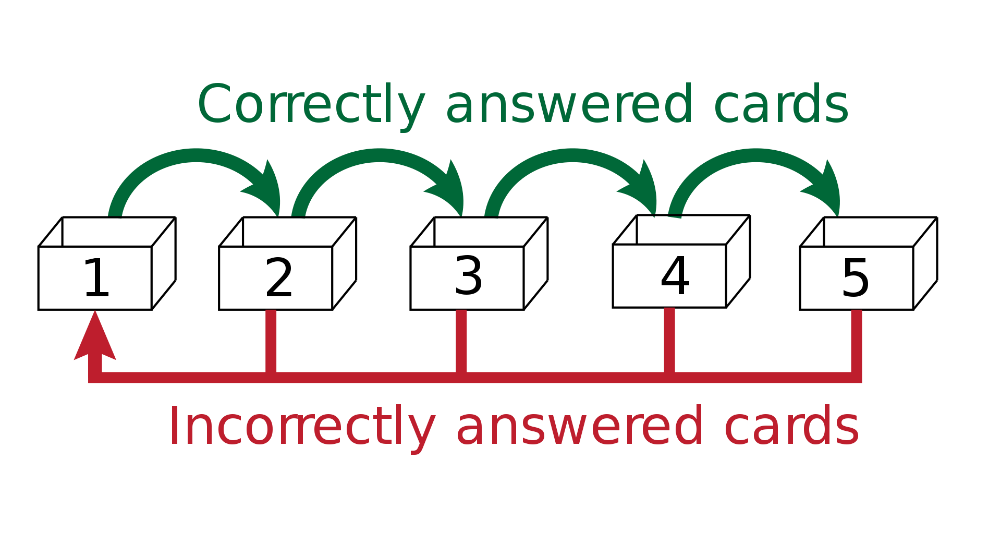
\includegraphics[scale=0.70]{leitner_system}
	\end{center}
	\legend{Fonte: Leitner System, 1970.}
\end{figure}


Durante os anos vários algoritmos foram desenvolvidos para otimizar o uso de flashcards nos estudos. Alguns dos métodos mais famosos são: Pimsleur, DASH e múltiplas versões do algoritmo SM. Para esse projeto o algoritmo escolhido para ser utilizado será o SM-2 que é o algoritmo de agendamento de \textit{flashcards} mais utilizado na indústria atualmente.

\section{CALL - Computer Assisted Language Learning}
CALL é a sigla para \textit{Computer Assisted Language Learning} ou “Aprendizado de Línguas Auxiliado por Computadores” (tradução livre) é um termo que vem sendo utilizado desde os anos 60. Michael Levy descreve em seu livro chamado \textit{Computer-Assisted Language Learning Context and Conceptualization} a origem e a natureza desse conceito e como softwares podem auxiliar professores e alunos ao aprender uma língua estrangeira. O autor argumenta que softwares não podem substituir todo o ensino da linguagem, o professor ainda tem um papel importante no ensino, contudo, softwares podem ser um grande fator auxiliar nessa tarefa já que permitem novas abordagens para o professor.

A partir desse conceito, George M. Chinnery cria o conceito de MALL (\textit{]Mobile Assisted Language Learning}) que em tradução livre pode ser lido como "Aprendizado de línguas auxiliado por dispositivos móveis". Considerando o número crescente de pessoas que utilizam smartphones e dispositivos móveis diariamente, faz sentido utilizar essas tecnologias a nosso favor e tornar o acesso ao aprendizado de línguas estrangeiras mais acessível. De acordo com Pesquisas feitas pelo \textit{Pew Research Center} (2011) apenas 35\% da população dos Estados Unidos possuíam um smartphone enquanto em 2019 esse número subiu para 81\%, ou seja, a maior parte da população norte-americana possui um dispositivo móvel que pode ser utilizado para o aprendizado de uma língua estrangeira.

\begin{figure}[H]
	\caption{\label{fig:smartphones}Quantidade da população que possui \textit{Smartphones}}
	\begin{center}
		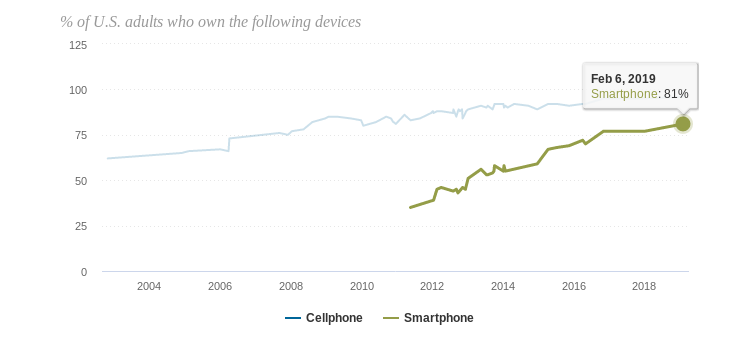
\includegraphics[scale=0.50]{smartphones}
	\end{center}
	\legend{Fonte: Disponível em: https://www.pewinternet.org/fact-sheet/mobile/. Acesso em: 30 set. 2019.}
\end{figure}

Em seu artigo \textit{Emerging Technologies - Going to the MALL: Mobile Assisted Language Learning}, Chinnery (2006) descreve que dispositivos móveis podem não ser a melhor plataforma para o aprendizado de novos conceitos, mas funcionam muito bem como uma ferramenta de revisão, o que colabora com o conceito inicial de CALL onde o software deve ser uma ferramenta de apoio para o estudante e não para substituir métodos tradicionais de ensino.

\section{Aprendizado Intencional De Vocabulário E Aprendizado Involuntário}
Ao aprender um novo vocabulário, um possível método de estudo é traduzir palavra por palavra através de sinônimos em sua língua nativa, esse método é chamado de aprendizado intencional de vocabulário ou aprendizado por substituição de palavras. Outra abordagem seria tentar inferir o significado da palavra dentro de um contexto, por exemplo ao ler o texto o leitor tenta através de outras palavras da frase interpretar ou pressupor o significado da palavra sem necessariamente achar uma palavra de referência em sua língua nativa, o nome dessa abordagem é aprendizado involuntário de vocabulário.

No artigo \textit{Intentional Vs. Incidental Vocabulary Learning} escrito por Jameel Ahmad (2012) o autor discursa sobre a efetividade de cada método ao se aprender novo vocabulário. As estatísticas fornecidas pelo estudo mostram que o método involuntário funciona significativamente melhor, pois requer do estudante um processo mental mais profundo e além de auxiliar na memorização de palavras também auxilia o aluno a reconhecer elementos semânticos da linguagem e associar como adjetivos e substantivos interagem na língua a ser estudada. Naturalmente não é sempre possível inferir o significado de uma palavra a partir do contexto, nesses casos deve-se utilizar o método de sinônimos.

Após a leitura desses estudos é possível concluir que utilizar \textit{flashcards} através de um sistema de repetição espaçada é bastante efetivo para aprender novo vocabulário, mas sua efetividade aumenta se utilizado dentro de um contexto textual onde é possível inferir o significado de algumas palavras, e quando não possível, as palavras com seus sinônimos na língua nativa podem ser adicionados ao sistema para melhor memorização.


